\documentclass[]{foi} 




\usepackage[utf8]{inputenc}
\usepackage[T1]{fontenc}
\usepackage{lipsum}
\usepackage{amsmath}
\usepackage{amssymb}
\usepackage{listings}
\usepackage{xcolor}
\usepackage{graphicx}
\usepackage{float}
\usepackage{longtable}
\usepackage{tikz}

\vrstaRada{\projekt}


\title{GENERIRANJE RAZINA IGRE KORI\v{S}TENJEM GRAMATIKE GRAFOVA}
\predmet{Deklarativno programiranje}


\author{Luka Kukec} 

\spolStudenta{\musko} 

\mentor{Bogdan Okreša Đurić}

\spolMentora{\musko} 

\titulaProfesora{doc.~dr.~sc.}

\godina{2026}
\mjesec{siječanj}

\indeks{0016158557}


\smjer{Baze podataka i baze znanja}

\sazetak{Ovaj rad opisuje implementaciju sustava za proceduralno generiranje razina u računalnim igrama koristeći gramatike grafova (engl. Graph Grammars). Sustav je implementiran u programskom jeziku Prolog s vizualizacijom u Pythonu (PyGame). Rad proučava teorijsku podlogu gramatika grafova i njihovu primjenu u stvaranju kompleksnih i varijabilnih struktura tamnica (dungeons).}


\kljucneRijeci{gramatike grafova; proceduralno generiranje sadržaja; Prolog; Python; razvoj igara; roguelike}


\acrodef{VAS}{višeagentni sustav}


\hypersetup{
    pdfencoding=auto,
    unicode=true
}

\begin{document}

\maketitle

\tableofcontents

\makeatletter \def\@dotsep{4.5} \makeatother
\pagestyle{plain}



\chapter{Uvod}
Računalne igre su kompleksni softverski sustavi koji zahtijevaju velike količine sadržaja kako bi održali interes igrača. Jedan od ključnih elemenata mnogih igara, posebno onih u žanru \textit{roguelike}, je dizajn razina. Ručno dizajniranje razina je vremenski zahtjevan proces koji ograničava količinu sadržaja koju razvojni tim može proizvesti. Kako bi se riješio ovaj problem, koristi se proceduralno generiranje sadržaja (engl. \textit{Procedural Content Generation - PCG}).

Ovaj rad bavi se proceduralnim generiranjem razina u igri korištenjem gramatika grafova (engl. \textit{Graph Grammars}). Motivacija za ovaj pristup leži u mogućnosti definiranja strukture razine putem skupa logičkih pravila, što omogućuje generiranje topološki ispravnih i zanimljivih tlocrta tamnica. Za razliku od jednostavnih nasumičnih algoritama, gramatike grafova nude bolju kontrolu nad strukturom i povezanošću prostorija \cite{dormans2010Adventures}.

Cilj rada je implementirati sustav koji koristi deklarativnu paradigmu (Prolog) za generiranje strukture razine na temelju gramatike, te imperativnu/objektno-orijentiranu paradigmu (Python) za vizualizaciju i interakciju s igračem.

\chapter{Teorijska podloga}

\section{Proceduralno generiranje sadržaja}
Proceduralno generiranje sadržaja (PCG) odnosi se na stvaranje sadržaja igre automatski, putem algoritama, s ograničenim ili neizravnim unosom korisnika \cite{togelius2011SearchBased}. PCG se koristi za generiranje različitih vrsta sadržaja, uključujući teksture, modele, glazbu, priču i razine \cite{adams2002AutomaticGeneration}. U kontekstu ovog rada, fokus je na generiranju razina, odnosno tlocrta prostora (tamnica).

Postoje različiti pristupi PCG-u, od jednostavnih nasumičnih algoritama do sofisticiranijih metoda poput gramatika grafova i L-sustava. Sustav Tanagra \cite{smith2011Tanagra} demonstrira kako se reaktivno planiranje može koristiti za interaktivni dizajn razina.

\section{Gramatike grafova}
Gramatike grafova su formalizam za specificiranje klasa grafova i operacija nad njima. Slično kao što Chomskyjeve gramatike definiraju pravila za generiranje nizova znakova (simbola), gramatike grafova definiraju pravila za generiranje grafova \cite{dormans2010Adventures}.

Gramatika grafa sastoji se od početnog grafa (aksioma) i skupa produkcijskih pravila (pravila prepisivanja). Svako pravilo definira podgraf koji se traži u trenutnom grafu (lijeva strana pravila) i podgraf kojim se on zamjenjuje (desna strana pravila).

Primjena gramatika grafova u generiranju razina omogućuje dizajnerima da definiraju "recepte" za strukturu razine \cite{rozenberg1997HandbookGraphGrammars}. Na primjer, pravilo može reći: "Ako postoji soba s blagom, dodaj sobu s čudovištem ispred nje". Ovo osigurava da generirane razine imaju smisla u kontekstu igrivosti (engl. \textit{gameplay}).

\section{L-sustavi}
L-sustavi (Lindenmayerovi sustavi) su paralelni sustavi za prepisivanje koji su originalno razvijeni za modeliranje rasta biljaka \cite{lindenmayer1968Mathematical}. Sastoje se od abecede simbola, aksioma (početnog niza) i skupa produkcijskih pravila. L-sustavi su srodne s gramatikama grafova i koriste se u proceduralnom generiranju za stvaranje fraktalnih i organskih struktura \cite{prusinkiewicz1990AlgorithmicBeauty}.

U kontekstu generiranja razina, L-sustavi mogu poslužiti za generiranje hodnika i povezivanje prostorija, dok gramatike grafova definiraju topološku strukturu tamnice.

\section{Logičko programiranje i Prolog}
Prolog (Programming in Logic) je deklarativni programski jezik koji se temelji na predikatnoj logici prvog reda \cite{bratko2012PrologProgramming}. Program u Prologu sastoji se od činjenica i pravila. Prolog je izuzetno pogodan za rješavanje problema koji uključuju simboličku manipulaciju, pretraživanje prostora stanja i zaključivanje, što ga čini idealnim alatom za implementaciju gramatika grafova.

U ovom radu Prolog se koristi za definiranje pravila gramatike i izvođenje procesa generiranja pretraživanjem i zamjenom simbola (čvorova grafa).

\section{Formalizacija sustava}
Kako bi se osigurala ispravnost i konzistentnost generiranih razina, sustav se može opisati formalnim jezikom predikatnog računa.

\subsection{Definicija predikata}
Osnovni građevni blokovi sustava definirani su sljedećim predikatima:
\begin{itemize}
    \item $room(id, x, y): \mathbb{N} \times \mathbb{Z} \times \mathbb{Z}$ -- Soba s jedinstvenim identifikatorom $id$ na koordinatama $(x,y)$.
    \item $connected(a, b, dir): \mathbb{N} \times \mathbb{N} \times Dir$ -- Soba $a$ povezana je sa sobom $b$ u smjeru $dir$, gdje je $Dir = \{north, south, east, west\}$.
    \item $room\_type(id, type): \mathbb{N} \times Type$ -- Soba $id$ je tipa $type$, gdje je $Type = \{start, boss, combat, treasure, shop, event\}$.
\end{itemize}

\subsection{Formalna pravila}
Sustav mora zadovoljiti skup logičkih ograničenja (constraints):

\textbf{Pravilo 1: Jedinstvenost početne i završne sobe}
Postoji točno jedna soba tipa \textit{start} i točno jedna soba tipa \textit{boss}.
\begin{equation}
    \exists! s \in Rooms: room\_type(s, start) \land \exists! b \in Rooms: room\_type(b, boss)
\end{equation}

\textbf{Pravilo 2: Povezanost grafa}
Za svake dvije sobe $r_1, r_2$ mora postojati put između njih.
\begin{equation}
    \forall r_1, r_2 \in Rooms: path(r_1, r_2)
\end{equation}

\textbf{Pravilo 3: Minimalna udaljenost}
Udaljenost između početne i završne sobe mora biti značajna (veća od ili jednaka 2).
\begin{equation}
    \forall s, b: (room\_type(s, start) \land room\_type(b, boss)) \implies distance(s, b) \geq 2
\end{equation}

\textbf{Pravilo 4: Topologija soba s blagom}
Sobe s blagom su "slijepoj ulici" (dead-end), odnosno imaju samo jedan izlaz.
\begin{equation}
    \forall r: room\_type(r, treasure) \implies degree(r) = 1
\end{equation}

Ovaj formalni model omogućuje tretiranje problema generiranja razine kao Problema zadovoljenja ograničenja (Constraint Satisfaction Problem - CSP), kojeg Prolog rješava mehanizmom unifikacije i backtrackinga.

\chapter{Opis implementacije}
Sustav se sastoji od dviju glavnih komponenti: generatora razina implementiranog u Prologu i grafičkog sučelja te logike igre implementiranih u Pythonu. Ove dvije komponente komuniciraju putem biblioteke \textit{pyswip} (ili subprocess poziva), gdje Python šalje zahtjev za generiranjem, a Prolog vraća strukturu razine.

\section{Arhitektura sustava}
Arhitektura je podijeljena na:
\begin{itemize}
    \item \textbf{Backend (Prolog)}: Odgovoran za logičko generiranje tlocrta tamnice, određivanje tipova soba i njihovih veza.
    \item \textbf{Frontend (Python/PyGame)}: Odgovoran za vizualizaciju, upravljanje stanjem igre (kretanje igrača, borba) i interakciju s korisnikom.
\end{itemize}

\begin{figure}[h!]
    \centering
    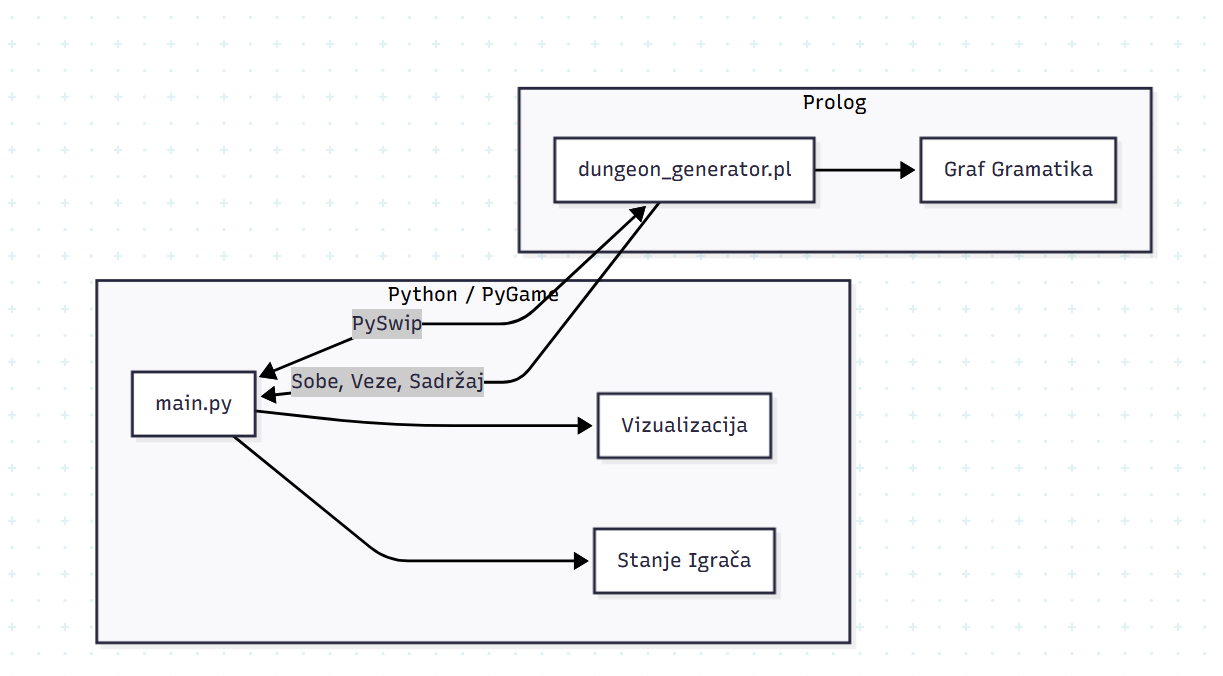
\includegraphics[width=0.9\textwidth]{slike/arhitektura_dijagram.png}
    \caption{Dijagram arhitekture sustava}
    \label{fig:architecture}
\end{figure}

\section{Generator u Prologu}
Jezgra generatora nalazi se u datoteci dungeon\_generator.pl. Generiranje započinje definiranjem gramatike grafa.

\subsection{Definicija gramatike}
Gramatika je definirana nizom pravila prepisivanja oblika weighted\_rule(ParentType, ChildType, Weight). Težina (weight) određuje relativnu vjerojatnost odabira tog tipa sobe. Primjer pravila iz koda:
\begin{lstlisting}[caption={Primjer gramatičkih pravila}, label={lst:grammar_rules}, language=Prolog, frame=single]
%% weighted_rule(ParentType, ChildType, Weight)

weighted_rule(start, combat, 60).
weighted_rule(start, event, 40).

weighted_rule(combat, combat, 50).
weighted_rule(combat, treasure, 30).
weighted_rule(combat, shop, 10).
weighted_rule(combat, event, 10).

weighted_rule(event, treasure, 40).
weighted_rule(event, empty, 30).
weighted_rule(event, combat, 30).

weighted_rule(empty, combat, 70).
weighted_rule(empty, event, 30).

weighted_rule(shop, combat, 100).

weighted_rule(treasure, boss, 60).
weighted_rule(treasure, combat, 40).

weighted_rule(boss, _, 0).
\end{lstlisting}

Ova pravila, prikazana u ispisu iznad, određuju koje nove sobe (čvorove) možemo stvoriti iz postojeće sobe određenog tipa. Veća težina znači veću vjerojatnost odabira - npr. shop ima samo 10\% šanse, dok combat ima 60\%.

\subsection{Probabilistička gramatika}
Za razliku od jednostavnih determinističkih gramatika, sustav koristi probabilističku gramatiku s težinama (engl. \textit{weighted rules}). Svako pravilo ima pridruženu težinu koja određuje vjerojatnost njegove primjene, kao što je prikazano u popisu iznad.

\subsection{Algoritam selekcije}
Odabir tipa sobe koristi \textit{roulette wheel} algoritam selekcije. Predikat select\_by\_weight/2 računa kumulativne težine i odabire tip proporcionalno njegovoj težini.

\subsection{Algoritam ekspanzije}
Proces generiranja koristi predikat expand\_dungeon/4 koji implementira pretraživanje u širinu (BFS) za širenje gramatike. Algoritam pokušava postaviti nove sobe na slobodne susjedne pozicije:

\begin{lstlisting}[caption={Algoritam ekspanzije tamnice}, label={lst:expansion_algo}, language=Prolog, frame=single]
%% expand_dungeon(Queue, Count, Max, Iterations)
expand_dungeon([room(ID, Type, X, Y) | RestQueue], Count, Max, Iterations) :-
    NewIterations is Iterations + 1,

    (   grammar_rule(Type, NextTypes) 
    ->  ShuffledTypes = NextTypes
    ;   ShuffledTypes = []
    ),
    
    spawn_neighbors(ID, X, Y, ShuffledTypes, RestQueue, NewQueue,
                    Count, NewCount, Max),
    expand_dungeon(NewQueue, NewCount, Max, NewIterations).

%% spawn_neighbors(...) pokušava postaviti sobe u nasumičnim smjerovima
spawn_neighbors(ParentID, X, Y, [NextType|RestTypes], 
                QueueIn, QueueOut, Count, FinalCount, Max) :-
    get_random_direction(DX, DY, Dir),
    NX is X + DX, NY is Y + DY,
    (   \+ claimed_pos(NX, NY)
    ->  NewCount is Count + 1,
        NewID = NewCount, 
        assertz(room(NewID, NX, NY)),
        assertz(room_type(NewID, NextType)),
        assertz(connected(ParentID, NewID, Dir)),
        assertz(claimed_pos(NX, NY)),
        opposite_dir_val(Dir, OppDir),
        assertz(connected(NewID, ParentID, OppDir)),
        NewQueueIn = [room(NewID, NextType, NX, NY) | QueueIn],
        spawn_neighbors(ParentID, X, Y, RestTypes, NewQueueIn, QueueOut,
                        NewCount, FinalCount, Max)
    ;   spawn_neighbors(ParentID, X, Y, RestTypes, QueueIn, QueueOut,
                        Count, FinalCount, Max)
    ).
\end{lstlisting}

Ovaj isječak koda prikazuje kako se rekurzivno širi struktura tamnice. Ključan je predikat spawn\_neighbors koji osigurava da se nove sobe ne preklapaju s postojećima provjerom claimed\_pos/2, a nasumičnost smjera postiže se permutacijom liste mogućih smjerova.
\newpage
\section{Integracija i Vizualizacija}
Python skripta pokreće Prolog generator i dohvaća rezultate u obliku liste soba i veza.
\begin{lstlisting}[caption={Integracija Pythona i Prologa}, label={lst:python_integration}, language=Python, frame=single]
def generate_dungeon(self, seed: int = 42, num_rooms: int = 7) -> dict:
    """ Generira dungeon pozivom Prologa. """
    query = f"generate_dungeon({seed}, {num_rooms}, Result)"
    results = list(self.prolog.query(query))
    
    if not results:
        raise RuntimeError("Prolog nije uspio generirati dungeon")
    
    return self._parse_dungeon_result(results[0]['Result'])
\end{lstlisting}
Kao što je prikazano u ispisu iznad, svaka soba se vizualizira kao pločica na ekranu, a hodnici (veze) se iscrtavaju između njih. Dodatno, sadržaj soba (neprijatelji, predmeti) se također generira u Prologu (generate\_room\_content/1) i prenosi u Python igru.

\chapter{Kritički osvrt}
Korištenje gramatika grafova pokazalo se kao robustan pristup za generiranje tamnica.

\section{Prednosti}
\begin{itemize}
    \item \textbf{Odvajanje strukture od algoritma}: Promjenom samo weighted\_rule predikata možemo drastično promijeniti topologiju tamnice (linearni hodnici vs. razgranati labirinti).
    \item \textbf{Fino podešavanje balansa}: Težine omogućuju kontrolu rijetkih soba (shop 10\%) bez mijenjanja algoritma.
    \item \textbf{Deklarativnost}: Prolog prirodno podržava backtracking što olakšava implementaciju ograničenja.
    \item \textbf{Modularnost}: Generator je potpuno odvojen od vizualizacije - može se koristiti s bilo kojim game engineom.
\end{itemize}

\section{Nedostaci}
\begin{itemize}
    \item \textbf{Složenost}: Potencijalna eksponencijalna složenost ako se pravila ne ograniče (riješeno s safety break od 500 iteracija).
    \item \textbf{Komunikacijski overhead}: PySwip sučelje između Pythona i Prologa uvodi određeno kašnjenje, iako za jednokratno generiranje to nije kritično.
    \item \textbf{Debugging}: Teže pronalaženje grešaka u Prolog kodu nego u imperativnim jezicima.
    \item \textbf{Ovisnost o SWI-Prologu}: Zahtijeva instalaciju Prologa na korisničkom sustavu.
\end{itemize}

\section{Mogući nastavak}
Projekt bi se mogao proširiti implementacijom lock-and-key mehanike, dinamičkim podešavanjem težine prema napretku igrača, ili vizualnim prikazom neprijatelja pomoću spriteova.

\chapter{Prikaz rada aplikacije}
U nastavku su prikazani primjeri generiranih tamnica.

\begin{figure}[h!]
    \centering
    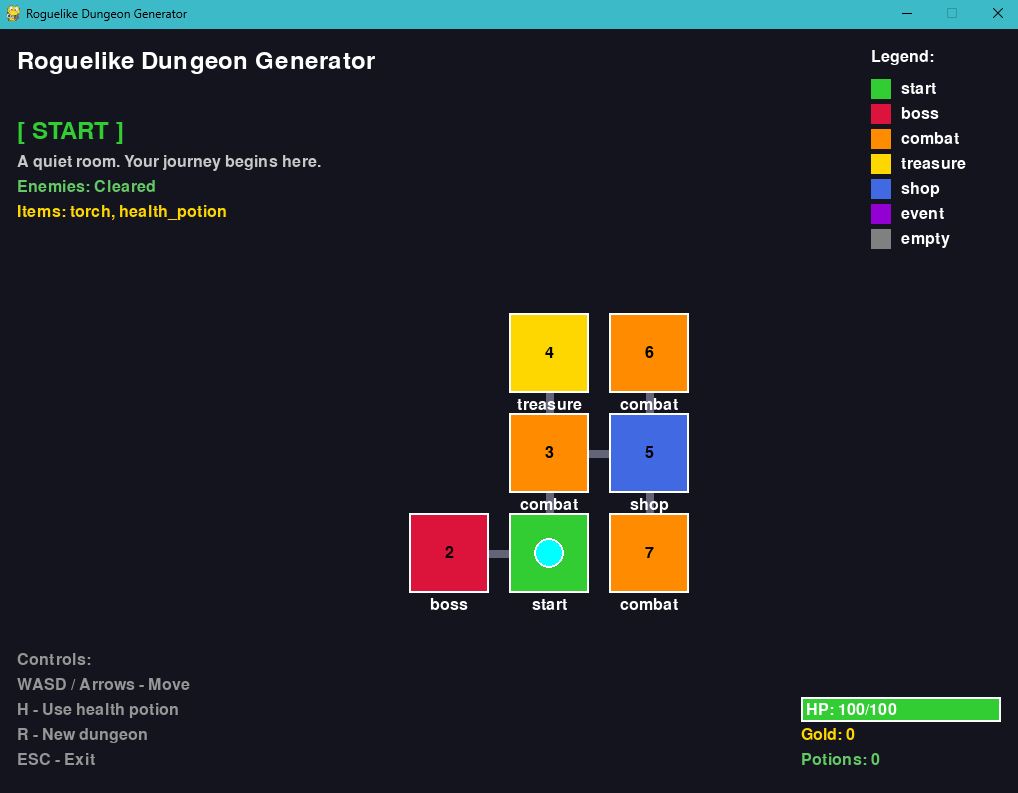
\includegraphics[width=0.8\textwidth]{slike/dungeon_example.png}
    \caption{Primjer generirane tamnice}
    \label{fig:dungeon_example}
\end{figure}

Aplikacija omogućuje igraču kretanje kroz generirane sobe, borbu s neprijateljima i skupljanje predmeta.

\chapter{Zaključak}
U ovom radu uspješno je implementiran sustav za proceduralno generiranje razina koristeći gramatike grafova u Prologu. Sustav demonstrira moć deklarativnog programiranja u rješavanju problema generiranja strukture. Iako postoje izazovi u integraciji s imperativnim jezicima, konačni rezultat je fleksibilan i proširiv generator koji može poslužiti kao temelj za složenije igre.

\makebackmatter
\end{document}
